\newpage
\chapter{Filling, Comparing and Normalizing Histograms using Macros (02/11/2016)}

With Python, it's quite easy to plot and slightly manipulate the contents of .root files. But once the analysis gets a bit more complicated (e.g., normalizing histograms), it's difficult to accomplish in Python because most of the stuff (like the classes and documentation) is written in/for C++. So for the time being, I'll be writing C++ macros rather than Python scripts for analysis.

With Bjoern's help, I created some macros to compare and analyse histograms. To be able to manipulate them for, e.g., normalizing, you have to create a new histogram and fill it with the contents of the branch/leaf you want to analyse because you can't edit the contents of a root file itself. All of this is difficult in Python, hence the switch to C++.

Three types of files were created: the header file (.h) which contains the information and declarations, etc., pertaining to the tree in the root file; the source file (.C) in which most of the analysis commands are executed; the "daddy" macro, which is what is executed in ROOT and ties the other source files and executes the necessary loops, etc.

As an example, I'm analysing the $\eta$ component of a jet from a \madgraph analysis from the processes $pp \rightarrow t\bar{t}$, $pp \rightarrow W +$ jets, and $pp \rightarrow Z +$ jets. These are SM backgrounds for a hadronic search because the DM final state is usually large \etmiss\ and several jets. The \madgraph output is converted into a .root file using my \textbf{rootconverter.sh} script. Then ROOT is launched and the analysis is done by executing the "daddy" macro (\textbf{execComparejets.C}) and I get a histogram out of it with three normalized plots of the respective Jet.Eta plots.

So in total I had 10 files used (daddy macro + $3\times3$ files for each analysis -- source file, header file, root file):

\begin{easylist}
\ListProperties(Style*=-- , FinalMark={)})
& execComparejets.C
& ppttbar.C \quad ppttbar.h \quad ppttbar.root
& ppWjets.C \quad ppWjets.h \quad ppWjets.root
& ppZjets.C \quad ppZjets.h \quad ppZjets.root
\end{easylist}

And the output file \textbf{comparejets.png}. At the moment, the aim is to plot SM background processes so we can find DM/exotic signals easier.

(Notes on \madgraph syntax can be found at \url{http://www.niu.edu/spmartin/madgraph/madsyntax.html}.)

The "daddy" macro \textbf{execComparejets.C}:

\lstinputlisting[language=C++, caption={A C++ macro designed to execute and loop over the macros tied to their respective root file. File name: execComparejets.C (v1).}]{./sec11/execComparejetsv1.C}

The C source file \textbf{ppttbar.C}:

\lstinputlisting[language=C++, caption={A C++ macro used to analyse the root file with the same name. A histogram is declared and filled with the Jet.Eta branch from the tree, then a histogram is drawn and normalised. File name: ppttbar.C (v1).}]{./sec11/ppttbarv1.C}

The header file \textbf{pptbar.h}:

%\href{run:./sec11/ppttbarv1.h}{ppttbar.h}:
The header file for the macro with the same name (ppttbar). I didn't display the file itself because the code stretches over 10 pages. This file includes all the declarations, branch names and other information relating to the root file. File name: ppttbar.h (v1).

The output \textbf{comparejets.png}:

\begin{figure}[H]
\centering
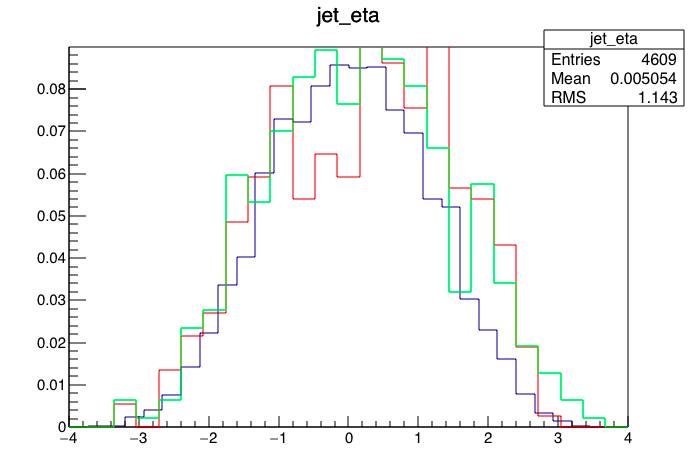
\includegraphics[width=\textwidth]{./sec11/comparejetsv1.png}
\caption{Multiple histograms showcasing the normalized entries versus pseudorapidity from three standard model processes: $pp \rightarrow t\bar{t}$ (blue); $pp \rightarrow W +$ jets (red); and $pp \rightarrow Z +$ jets (green).}
\end{figure}

I should find a way to plot such that the histogram with the largest $y$-value is plotted first. So for the time being, until I can streamline it, the process for getting and analysing data is as follows:

\begin{easylist}[enumerate]
& Write an input file for \madgraph detailing the process I want to look at.
& Run \madgraph with the input file and get the output .lhco files, etc.
& Convert the .lhco and .lhe files to .root files using my rootconverter.sh script.
& Run ROOT and get the MakeClass file (.h and .C) for the .root file.
& Use the templates above to edit the .h and .C files accordingly, paying close attention to the other header files I need to include, the bin sizes of the histograms, the names of the branches I'm accessing, normalization, line colours, whether the histogram is cut off because of the canvas size.
& Write the "daddy" macro to execute and run all the analyses and get the histogram(s) out.
\end{easylist}

\textbf{UPDATE:} As a start to the streamlining process, I wrote a header file \textbf{global.h} which is intended to store global variables/constants, etc., and also all my "include" headers. At the time of writing I've only included the ranges and number of bins for initialising histograms (because for now I'll be plotting the same type of histogram in one graph, so it makes sense that they all have the same range and number of bins), and the "include" headers (so in each file I only have to include global.h and the C++ source files that are tied to it). Hopefully I'll be able to expand this to include the names of the histograms and cut variables (as character strings?) so that they only have to be declared once and I only have to edit one line if I want to plot something else/apply a different cut. The current version of global.h is presented below:

\lstinputlisting[language=C++, caption={The global header file to include global variables/constants/headers that my C++ macros need. File name: global.h (v1).}]{./sec11/globalv1.h}

\begin{figure}[H]
\centering
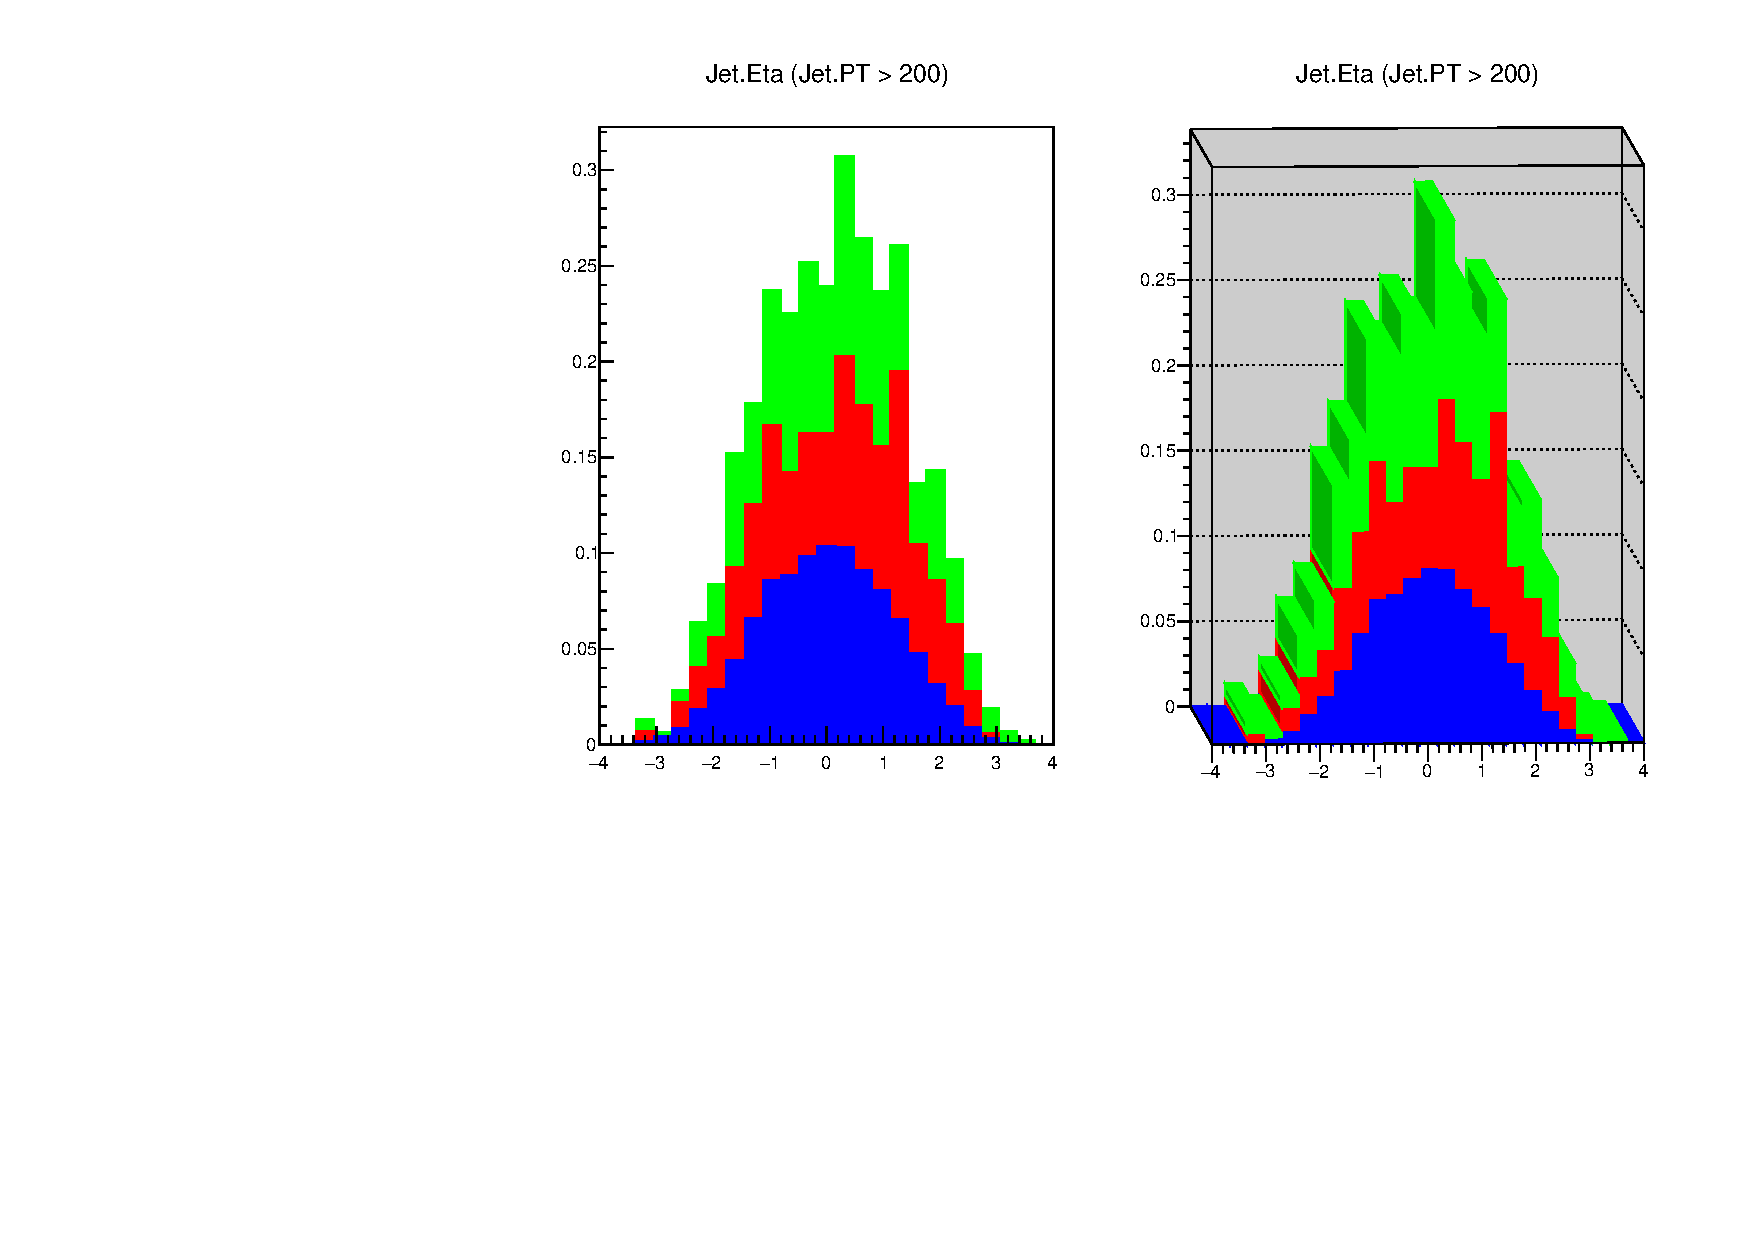
\includegraphics[width=\textwidth]{./sec11/comparejetsv2.pdf}
\cprotect\caption{Multiple histograms showcasing the normalized entries versus pseudorapidity from three standard model processes: $pp \rightarrow t\bar{t}$ (blue); $pp \rightarrow W +$ jets (red); and $pp \rightarrow Z +$ jets (green). These were plotted as a histogram stack. The left panel is from the base \texttt{Draw()} command in ROOT, and the right panel displays the same stack as a "lego" plot.}
\end{figure}

I've updated my macros slightly to divide the canvas and make a "lego" plot that's angled slightly to give a different perspective. Both plots were created using the \texttt{THStack} class so that the histograms can be added and then plotted as a stack so you don't get any weird overlap like you do when plotting them one-by-one. I haven't updated the code enough to justify sticking it in the lab book. Maybe I'll add it once I've figured out how to add the legend and added some other features.

\textbf{UPDATE:} I've figured out how to add legends to the plots and have tidied up/expanded some of the files. I might add the new versions of the code later on.

\section{Updated code for C++ macros}

An updated version (v3) of my files are included below (but not in my physical lab book for waste of time and paper) for future reference. The header files are not included because they have not changed, and are the same across all three processes with the exception of the function names and the names of the .root files. The update notes: more parameters and include files being held in \textbf{global.h}; the canvas declaration and some aesthetics being executed by the "daddy" macro; a legend; and scaling by luminosity instead of area.

The "daddy" macro:

\lstinputlisting[language=C++, caption={The C++ macro used to execute the macros pertaining to the individual root files, but updated and streamlined. File name: execComparejets.C (v3).}]{./sec11/execComparejetsv3.C}

The global header file \textbf{global.h}:

\lstinputlisting[language=C++, caption={The global header file that includes some declarations, global variables/constants/include files, but updated and streamlined. File name: global.h (v3).}]{./sec11/globalv3.h}

The source file \textbf{ppttbar.C}:

\lstinputlisting[language=C++, caption={The C++ macro used to analyse ppttbar.root, but updated and streamlined. File name: ppttbar.C (v3).}]{./sec11/ppttbarv3.C}

The source file \textbf{ppWjets.C}:

\lstinputlisting[language=C++, caption={The C++ macro used to analyse ppWjets.root, but updated and streamlined. File name: ppWjets.C (v3).}]{./sec11/ppWjetsv3.C}

The source file \textbf{ppZjets.C}:

\lstinputlisting[language=C++, caption={The C++ macro used to analyse ppZjets.root, but updated and streamlined. File name: ppZjets.C (v3).}]{./sec11/ppZjetsv3.C}

The output file \textbf{comparejets.pdf}:

\begin{figure}[H]
\centering
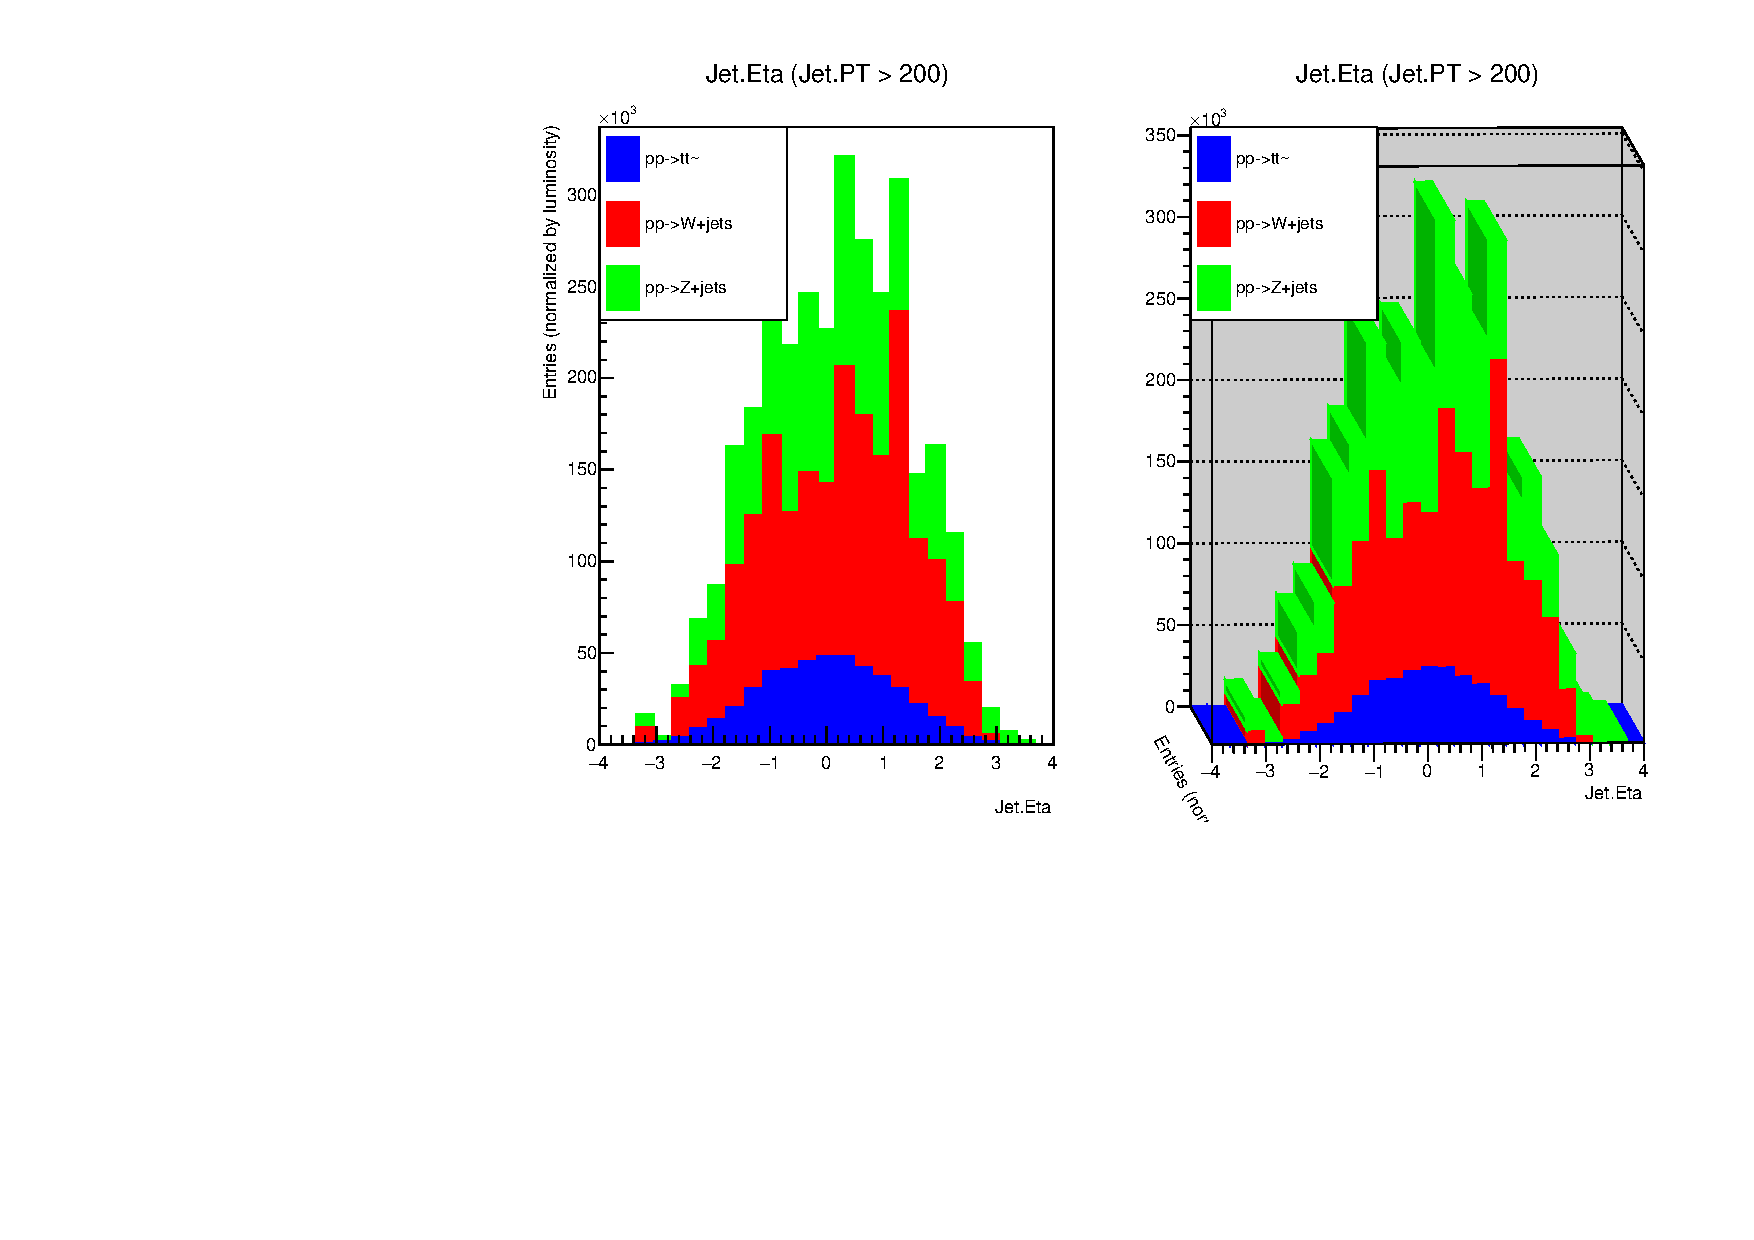
\includegraphics[width=\textwidth]{./sec11/comparejetsv3.pdf}
\caption{The same histograms from the previous subsection plotted as a histogram stack, this time with a legend and axis labels. The entries are also normalized by luminosity rather than area.}
\end{figure}

In this version of the code, each histogram was normalized according to the luminosity. The scale factor $s.f.$ was calculated using the simple, standard formula

\begin{equation}
\label{eq:lumiexpev}
N = \sigma \mathcal{L}
\end{equation}

where $N$ is the number of events, $\sigma$ is the interaction cross section, and $\mathcal{L}$ is the luminosity. These values are detailed in Table \ref{tab:comparison}. Then the scale factor is

\begin{equation}
s.f. = \sigma \mathcal{L} / N
\end{equation}

and is dimensionless, since [$\sigma$] = pb and [$\mathcal{L}$] = pb$^{-1}$.

\begin{table}[H]
\centering
    \begin{tabular}{|l|l|l|l|}
    \hline
    Property                                & $pp \rightarrow t\bar{t}$ & $pp \rightarrow W + \mathrm{jets}$ & $pp \rightarrow Z^0 + \mathrm{jets}$ \\ \hline
    Number of Events (MadGraph)             & 100 000 & 100 000 & 100 000 \\
    Cross section (pb)                      & 504.9   & $2.144\times10^4$ & $1.166\times10^4$ \\
    Assumed luminosity (pb$^{-1}$)		& 20 000	& 20 000 & 20 000 \\
    Jet $\eta$ events before cut               & 99 999  & 99 992  & 99 996  \\
    Jet $\eta$  events after cut (Jet $p_{\mathrm{T}} >$ 200) & 4 609    & 371     & 470     \\
    Efficiency (\%)                         & 4.6     & 0.37    & 0.47    \\ \hline
    \end{tabular}
\caption{The properties of the \madgraph processes that were simulated.}
\label{tab:comparison}
\end{table}

The luminosity from a process is given in the stream of output text during a \madgraph run, but I didn't realise until after I had made the plots. So I just assumed the luminosity was 20 fb$^{-1}$ (20,000 pb$^{-1}$). The luminosity would most likely be different for each decay and so would scale the histograms slightly differently, but the point of this exercise was to demonstrate the technique behind filling and plotting histograms rather than a rigorous analysis. The efficiency was just calculated from the number of events after the cut $\div$ number before the cut.

\section{Running \madgraph for benchmarks}

I've run a few different simulations in \madgraph to get benchmark times to see which processes are the most efficient, possibly for future backgrounds or analyses. The following processes (with the names of the output files) in terms of \madgraph syntax were run with 10,000 events. Bottom quarks and tau leptons were also included in the multiparticle labels in the input files. Some processes included Quantum Chromodynamics (QCD) at Next to Leading Order (NLO) and ran their own subprocesses within \madgraph. All other settings were left as their default.

\begin{lstlisting}[belowskip=-0.7cm, language=sh, numbers=none]
generate p p > t t~, (t > b W+, W+ > l+ vl), (t~ > b~ W-, W- > s c~)
output ttbar_onshell_nomerging

generate p p > t t~ [QCD]
output ttbar_onshell_NLO

generate p p > W+
add process p p > W+ j
add process p p > W+ j j
output W_multijets

decay Z > b b~
decay Z > vl vl~
generate p p > Z W- [QCD]
output WmZ_NLO

generate p p > Z W-
add process p p > Z W- j
output WmZj

decay Z > b b~
decay Z > vl vl~
generate p p > Z W+ [QCD]
output WpZ_NLO

generate p p > Z W+
add process p p > Z W+ j
output WpZj

generate p p > Z
add process p p > Z j
add process p p > Z j j
output Z_simplejetmerging

generate p p > Z, (Z > vl vl~)
add process p p > Z j, (Z > vl vl~)
add process p p > Z j j, (Z > vl vl~)
output Zjets_invisible

generate p p > Z Z [QCD]
output ZZ_NLO

generate p p > Z Z
add process p p > Z Z j
output ZZjets
\end{lstlisting}

\

The results are displayed below.

\lstinputlisting[language=sh, caption={Benchmark run times for different processes executed in \madgraph. File name: process\texttt{\char`_}comparison.txt}.]{./sec11/process_comparison.txt}

The NLO processes automatically set the number of events to 10,000 and give me an error message if I use the command \texttt{set nevents ...}, so I set the number of events to 10,000 for all runs. \PYTHIA and PGS were \texttt{OFF}, but the NLO processes run their own extra routines, like \textsc{MCatNLO} and HERWIG6.

To compare the cross sections I got with the currently accepted values, see \url{https://twiki.cern.ch/twiki/bin/viewauth/CMS/SummaryTable1G25ns}.
